\section{MO-teori og hybridisering}
I molekylær orbital teori ses der på fordelingen af elektroner i molekyler på samme måde som vi ser på fordelingen af elektroner i atomer.\refUniphys{186}) Måden hvorpå vi bestemmer hvordan en elektron opfører sig på i et molekyle er ved hjælp af kvantemekanik og en bølgefunktion $\Psi$.\refUniKemi{149} På denne måde kan energien af en elektron og formen på det område hvori en elektron bevæger sig i bestemmes. Som vi i afsnit \ref{elektroner} fandt ud af, havde elektroner nogle områder hvori de havde den størst mulige change for at blive fundet i. Disse områder kaldte vi orbitaler. Som enkelte atomer har orbitaler, har molekyler ligeledes orbitaler hvori elektronerne har en stor chance for at blive fundet i. Forskellen på atomer og molekyler er, at elektroner i molekyler kan findes nær en hvilken som helst kerne i molekylet i stedet for den ene kerne, som orbitalen hører til for et atom.\refUniKemi{149} Dette er netop hvorfor vi kalder disse orbitaler for molekylære elektronorbitaler eller bare molekylære orbitaler. Ligesom atomare orbitaler er molekyære orbitaler også fyldt når de indeholder præcist 2 orbitaler med modsat spin. 
\\

\begin{wrapfigure}{r}{0.55\textwidth}
  \centering
  \begin{tikzpicture}[scale=1.5]
  \begin{scope}[font=\itshape]% 

  \draw[-latex] (0,-1)--(0,1) node[above]{Stigende energi};
  \orbital[color = purple, opacity = 1, scale = 2, pos = {(1,0.65)}]{s} 
  \orbital[color = purple, opacity = 1, scale = 2, pos = {(2,0.65)}]{s} 
  \node[above] at (1,0.5) {+};  
  \node[above] at (2,0.5) {+};
  \node[above] at (0.9,-0.15) {s orbital};
  \node[above] at (2.1,-0.15) {s orbital};
	\draw[-latex] (2.5,0.65)--(3.5,-0.10);
 		
 		
 		
 \orbital[color = purple, opacity = 0.2, scale = 2, pos = {(4,-0.5)}]{s} 
  \orbital[color = purple, opacity = 0.2, scale = 2, pos = {(4.5,-0.5)}]{s}  	
  	
  \node[above] at (4.2,-1.5) {Bindende orbital $\sigma_s$};
 	\node[above] at (4,-0.65) {+}; 
 	\node[above] at (4.5,-0.65) {+}; 
  \end{scope}

  \begin{pgfonlayer}{backbackground}
  \fill[white](current bounding box.south west)rectangle
  (current bounding box.north east);
  \end{pgfonlayer}
  \end{tikzpicture}
  \caption{Sigma-binding \label{fig:sigmabinding}}
   \end{wrapfigure}

Da vi så de atomare orbitaler gav vi dem navnene, s,p,d og f. Molekylære orbitaler har også navne, men der vil i denne opgave ligge et fokus på $\pi$-orbitaler og $\sigma$-orbitaler. Lad os som eksempel betragte et eksempel på et homonukleært diatomisk molekyle som $H_2$. De to hydrogenatomer der er bundet sammen har hver deres egen elektron, men når de er tilpas tæt nok på hinanden vil elektronerne i deres 1s orbitaler overlappe. Da elektronerne er negativt ladede og de 2 hydrogenkerner er positivt ladede, vil elektronerne blive tiltrukket af begge kerner og have et lavere niveau af energi ved at befinde sig mellem de to atomer end de ville have isolerede.\refUniKemi{151} Elektronerne vil altså søge at befinde sig mellem de to kerner og derved stabilisere molekylet. Denne slags orbitaler kaldes \textbf{bindende} orbitaler, da de som navnet antyder binder molekylet sammen. Da der stadigvæk kun er plads til 2  elektroner i en orbital, vil elektroner der ikke kan indgå i bindende orbitaler indgå i anti-bindende orbitaler. Disse orbitaler er med til at destabilisere molekyler og er en af grundene til at alle atomer kan gå i forbindelse med hinanden. De anti-bindende orbitaler findes ved at tage to orbitaler der overlapper hinanden og fjerne deres overlap. Nu er orbitalen ikke mellem atomerne mere og vil derfor ikke stabilisere molekylet længere. På figur\ref{fig:sigmabinding} er det illustreret hvordan to atomare orbitaler går sammen om at danne en bindende $\sigma_s$ orbital. 
\\

Når to atomare orbitaler går sammen om at danne en ny orbital kalder vi det en hybridisering. En $\sigma$-binding er altså en hybridorbital.
\\

En $\sigma$-orbital er også det vi kender som en $\sigma$-binding eller en slags kovalent binding. Kovalente bindinger er defineret som molekylære bindinger, der involverer en deling af elektroner mellem to atomer.\refUniKemi{151}
\\

På samme måde som med $\sigma$-orbitalerne dannes $\pi$-orbitalerne ved, at to atomers befinder sig tæt på hinanden og elektronerne kan få en lavere energi ved at befinde sig i det sted hvor orbitalerne overlapper. Det græske bogstav $\pi$ refererer til p-orbitalerne. Dette er fordi $\pi$-orbitaler oftest ses dannet ud fra netop p-orbitaler, men det skal sige, at de også kan dannes ud fra d orbitaler. På figur \ref{fig:ethen} ses hvordan 2 p-orbitaler går sammen om at danne en $\pi$-bindinger. 
	
Nu har vi set på både $\sigma$-orbitaler /bindinger og $\pi$-orbitaler / bindinger - men hver for sig. Hvis de to orbitaler eksisterer sammentidigt i et molekyle har vi faktisk en dobbeltbinding. Dobbeltbindinger er netop en $\sigma$- og en $\pi$-binding. Illustret som en tegning ville det se ud på følgende måde, se Figur \ref{fig:ethen}.

\begin{wrapfigure}{r}{0.5\textwidth}
\begin{center}
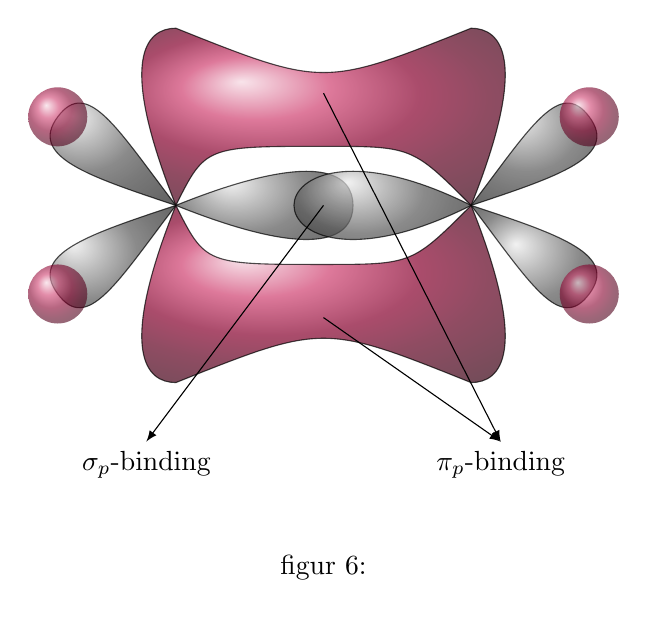
\begin{tikzpicture}[scale=0.75]

\shade[shading=ball, ball color=gray,draw,opacity=.7] (-2.5,0) .. controls (0,1) and     (.5,0.5) .. (.5,0)
.. controls (.5,-.5) and (0,-1) .. (-2.5,0);

\shade[shading=ball, ball color=gray,draw,opacity=.7] (2.5,0) .. controls (.5,1) and     (-.5,0.5) .. (-.5,0)
.. controls (-.5,-.5) and (.5,-1) .. (2.5,0);


\shade[shading=ball, ball color=gray,draw,opacity=.7] (-2.5,0) .. controls (-4,0.5) and     (-5,0.83) .. (-4.5,1.5)
.. controls (-4,2.17) and (-3.5,1.31) .. (-2.5,0);

\shade[shading=ball, ball color=gray,draw,opacity=.7] (-2.5,0) .. controls (-4,-0.5)     and (-5,-0.83) .. (-4.5,-1.5)
.. controls (-4,-2.17) and (-3.5,-1.31) .. (-2.5,0);


\shade[shading=ball, ball color=gray,draw,opacity=.7] (2.5,0) .. controls (4,0.5) and     (5,0.83) .. (4.5,1.5)
.. controls (4,2.17) and (3.5,1.31) .. (2.5,0);

\shade[shading=ball, ball color=gray,draw,opacity=.7] (2.5,0) .. controls (4,-0.5) and     (5,-0.83) .. (4.5,-1.5)
.. controls (4,-2.17) and (3.5,-1.31) .. (2.5,0);

\shade[shading=ball, ball color=purple,opacity=0.6] (4.5,1.5) circle (0.5);

\shade[shading=ball, ball color=purple,opacity=0.6] (4.5,-1.5) circle (.5);

\shade[shading=ball, ball color=purple,opacity=0.6] (-4.5,-1.5) circle (.5);

\shade[shading=ball, ball color=purple,opacity=0.6] (-4.5,1.5) circle (.5);


\shade[shading=ball, ball color=purple,draw,opacity=.7] (-2.5,0) .. controls (-3.5,2.5)     and (-3,3) .. (-2.5,3)
.. controls (0,2) .. (2.5,3)
.. controls (3,3) and (3.5,2.5) .. (2.5,0)
.. controls (1.5,1) .. (0,1)
.. controls (-2,1) .. (-2.5,0);


\shade[shading=ball, ball color=purple,draw,opacity=.7] (-2.5,0) .. controls (-3.5,-2.5)     and (-3,-3) .. (-2.5,-3)
.. controls (0,-2) .. (2.5,-3)
.. controls (3,-3) and (3.5,-2.5) .. (2.5,-0)
.. controls (1.5,-1) .. (0,-1)
.. controls (-2,-1) .. (-2.5,-0);

\draw[-latex] (0,0)--(-3,-4) node[below]{$\sigma_p$-binding};

\draw[-latex] (0,1.9)--(3,-4) node[below]{$\pi_p$-binding};

\draw[-latex] (0,-1.9)--(3,-4) node[below]{ };


\node[above] at (0,-6.5){figur 6: };
\end{tikzpicture}
\end{center}
\caption{Orbitaler i ethen \label{fig:ethen}}
\end{wrapfigure}

$\sigma$-bindingerne er de stærkestee af de kovalente bindinger. Dernæst kommer $\pi$-bindingerne. blabla MO teori...


Det er nemmelig ikke alle atomer, der har mulighed for at danne kovalente bindinger imellem sig. Når 2 atomer går sammen om at danne en kovalent binding er det fordi, at de hver især er ustabile. At de er ustabile er ens betydende med, at de ikke har deres orbitaler af højeste energiniveau fyldt ud. Hver orbital vil gerne have en spin-op og en spin-ned elektron. Når nogle atomer så alligevel ikke vælger at gå sammen og danne en kovalent binding er det enten fordi, at de har for mange mange elektroner til, at de kun kan befinde sig mellem atomerne og danne en bindende $\sigma$-binding og derfor befinder sig i en orbital, der kræver et højere energiniveau og derfor er anti-bindende. 


